% GNUPLOT: LaTeX picture with Postscript
\begingroup
  \makeatletter
  \providecommand\color[2][]{%
    \GenericError{(gnuplot) \space\space\space\@spaces}{%
      Package color not loaded in conjunction with
      terminal option `colourtext'%
    }{See the gnuplot documentation for explanation.%
    }{Either use 'blacktext' in gnuplot or load the package
      color.sty in LaTeX.}%
    \renewcommand\color[2][]{}%
  }%
  \providecommand\includegraphics[2][]{%
    \GenericError{(gnuplot) \space\space\space\@spaces}{%
      Package graphicx or graphics not loaded%
    }{See the gnuplot documentation for explanation.%
    }{The gnuplot epslatex terminal needs graphicx.sty or graphics.sty.}%
    \renewcommand\includegraphics[2][]{}%
  }%
  \providecommand\rotatebox[2]{#2}%
  \@ifundefined{ifGPcolor}{%
    \newif\ifGPcolor
    \GPcolortrue
  }{}%
  \@ifundefined{ifGPblacktext}{%
    \newif\ifGPblacktext
    \GPblacktextfalse
  }{}%
  % define a \g@addto@macro without @ in the name:
  \let\gplgaddtomacro\g@addto@macro
  % define empty templates for all commands taking text:
  \gdef\gplbacktext{}%
  \gdef\gplfronttext{}%
  \makeatother
  \ifGPblacktext
    % no textcolor at all
    \def\colorrgb#1{}%
    \def\colorgray#1{}%
  \else
    % gray or color?
    \ifGPcolor
      \def\colorrgb#1{\color[rgb]{#1}}%
      \def\colorgray#1{\color[gray]{#1}}%
      \expandafter\def\csname LTw\endcsname{\color{white}}%
      \expandafter\def\csname LTb\endcsname{\color{black}}%
      \expandafter\def\csname LTa\endcsname{\color{black}}%
      \expandafter\def\csname LT0\endcsname{\color[rgb]{1,0,0}}%
      \expandafter\def\csname LT1\endcsname{\color[rgb]{0,1,0}}%
      \expandafter\def\csname LT2\endcsname{\color[rgb]{0,0,1}}%
      \expandafter\def\csname LT3\endcsname{\color[rgb]{1,0,1}}%
      \expandafter\def\csname LT4\endcsname{\color[rgb]{0,1,1}}%
      \expandafter\def\csname LT5\endcsname{\color[rgb]{1,1,0}}%
      \expandafter\def\csname LT6\endcsname{\color[rgb]{0,0,0}}%
      \expandafter\def\csname LT7\endcsname{\color[rgb]{1,0.3,0}}%
      \expandafter\def\csname LT8\endcsname{\color[rgb]{0.5,0.5,0.5}}%
    \else
      % gray
      \def\colorrgb#1{\color{black}}%
      \def\colorgray#1{\color[gray]{#1}}%
      \expandafter\def\csname LTw\endcsname{\color{white}}%
      \expandafter\def\csname LTb\endcsname{\color{black}}%
      \expandafter\def\csname LTa\endcsname{\color{black}}%
      \expandafter\def\csname LT0\endcsname{\color{black}}%
      \expandafter\def\csname LT1\endcsname{\color{black}}%
      \expandafter\def\csname LT2\endcsname{\color{black}}%
      \expandafter\def\csname LT3\endcsname{\color{black}}%
      \expandafter\def\csname LT4\endcsname{\color{black}}%
      \expandafter\def\csname LT5\endcsname{\color{black}}%
      \expandafter\def\csname LT6\endcsname{\color{black}}%
      \expandafter\def\csname LT7\endcsname{\color{black}}%
      \expandafter\def\csname LT8\endcsname{\color{black}}%
    \fi
  \fi
    \setlength{\unitlength}{0.0500bp}%
    \ifx\gptboxheight\undefined%
      \newlength{\gptboxheight}%
      \newlength{\gptboxwidth}%
      \newsavebox{\gptboxtext}%
    \fi%
    \setlength{\fboxrule}{0.5pt}%
    \setlength{\fboxsep}{1pt}%
\begin{picture}(8502.00,4534.00)%
    \gplgaddtomacro\gplbacktext{%
      \csname LTb\endcsname%
      \put(550,815){\makebox(0,0)[r]{\strut{}$0$}}%
      \csname LTb\endcsname%
      \put(550,1239){\makebox(0,0)[r]{\strut{}$5$}}%
      \csname LTb\endcsname%
      \put(550,1663){\makebox(0,0)[r]{\strut{}$10$}}%
      \csname LTb\endcsname%
      \put(550,2087){\makebox(0,0)[r]{\strut{}$15$}}%
      \csname LTb\endcsname%
      \put(550,2511){\makebox(0,0)[r]{\strut{}$20$}}%
      \csname LTb\endcsname%
      \put(550,2935){\makebox(0,0)[r]{\strut{}$25$}}%
      \csname LTb\endcsname%
      \put(550,3359){\makebox(0,0)[r]{\strut{}$30$}}%
      \csname LTb\endcsname%
      \put(550,3783){\makebox(0,0)[r]{\strut{}$35$}}%
      \csname LTb\endcsname%
      \put(550,4206){\makebox(0,0)[r]{\strut{}$40$}}%
      \csname LTb\endcsname%
      \put(682,484){\makebox(0,0){\strut{}$0$}}%
      \csname LTb\endcsname%
      \put(1456,484){\makebox(0,0){\strut{}$2$}}%
      \csname LTb\endcsname%
      \put(2230,484){\makebox(0,0){\strut{}$4$}}%
      \csname LTb\endcsname%
      \put(3004,484){\makebox(0,0){\strut{}$6$}}%
      \csname LTb\endcsname%
      \put(3778,484){\makebox(0,0){\strut{}$8$}}%
      \csname LTb\endcsname%
      \put(4552,484){\makebox(0,0){\strut{}$10$}}%
      \csname LTb\endcsname%
      \put(5326,484){\makebox(0,0){\strut{}$12$}}%
      \csname LTb\endcsname%
      \put(6100,484){\makebox(0,0){\strut{}$14$}}%
      \put(6425,4187){\makebox(0,0)[l]{\strut{}$1.2$}}%
      \put(6425,3202){\makebox(0,0)[l]{\strut{}$2$}}%
      \put(6425,1864){\makebox(0,0)[l]{\strut{}$4$}}%
      \put(6425,785){\makebox(0,0)[l]{\strut{}$7$}}%
    }%
    \gplgaddtomacro\gplfronttext{%
      \csname LTb\endcsname%
      \put(176,2486){\rotatebox{-270}{\makebox(0,0){\strut{}Particle Mass Concentration / $\%$}}}%
      \put(6732,2486){\rotatebox{270}{\makebox(0,0){\strut{}X-ray Transmission / $\%$}}}%
      \put(3487,154){\makebox(0,0){\strut{}Vertical Position / mm}}%
      \csname LTb\endcsname%
      \put(7505,704){\makebox(0,0)[l]{\strut{}\smaller 100}}%
      \put(7505,1213){\makebox(0,0)[l]{\strut{}\smaller 120}}%
      \put(7505,1722){\makebox(0,0)[l]{\strut{}\smaller 140}}%
      \put(7505,2231){\makebox(0,0)[l]{\strut{}\smaller 160}}%
      \put(7505,2741){\makebox(0,0)[l]{\strut{}\smaller 180}}%
      \put(7505,3250){\makebox(0,0)[l]{\strut{}\smaller 200}}%
      \put(7505,3759){\makebox(0,0)[l]{\strut{}\smaller 220}}%
      \put(7505,4269){\makebox(0,0)[l]{\strut{}\smaller 240}}%
      \put(7968,2486){\rotatebox{270}{\makebox(0,0){\strut{}\smaller Diffusion Time / min}}}%
    }%
    \gplbacktext
    \put(0,0){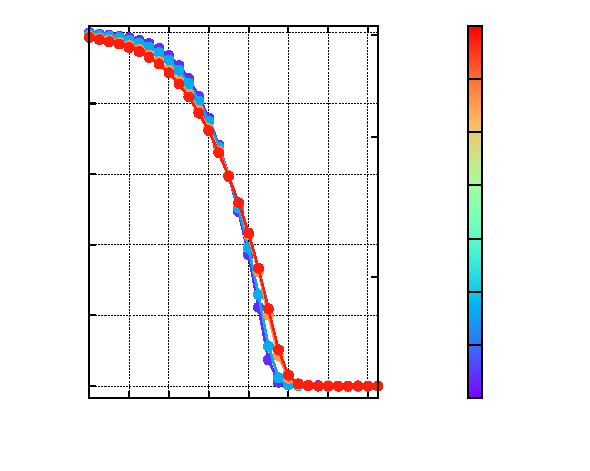
\includegraphics{LudoxHS40TransmissionCalibration}}%
    \gplfronttext
  \end{picture}%
\endgroup
